\chapter{Introduction} \label{sec:Introduction}

\section{Big Picture} \label{intro:sec:bigpicture}




\begin{figure}[H]
    \centering
    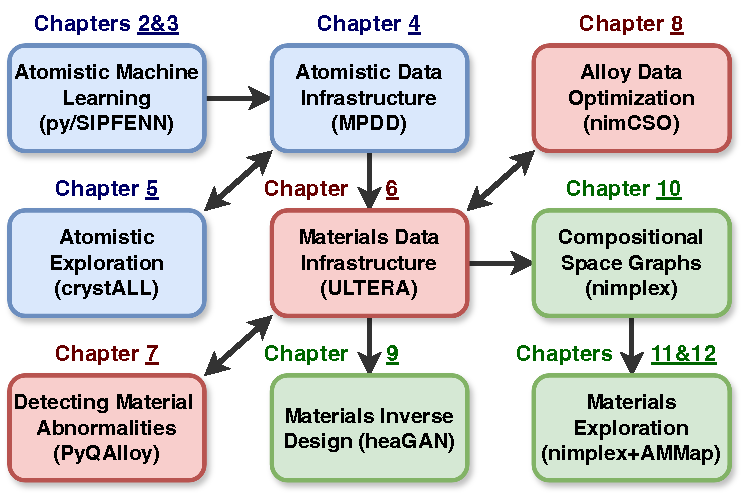
\includegraphics[width=0.7\textwidth]{intro/DissertationOutline.pdf}
    \caption{
    Jet engine photo from Olivier Cleynen under CC
    Hypersonic vehicle render by DARPA from public domain.
    }
    \label{intro:fig:outline}
\end{figure}

Per DOE ARPA-E estimates, developing a standalone alloy which could continuously operate at $1300^oC$ has the potential to increase gas turbine efficiency up to 7\%, which will significantly reduce wasted energy and carbon emissions by saving up to 20 quads of energy in electricity generation and civilian aviation between now and 2050 \cite{ULTIMATEArpa-e.energy.gov}. Such efficiency increase could prevent release of approximately 1,000,000,000,000 kg of \ch{CO_2} from burning natural gas, or double that from coal.


Another extreme environment application is the class of hypersonic vehicles which travel faster than 5 times the speed of sound \emph{through Earth's atmosphere for extended periods of time}, thus, generating extreme sustained temperatures within structural components. This prompts the need for novel materials and engineering techniques, as evidenced by massive funding assigned to this research areas by United States military which increased its yearly budgets for hypersonic \emph{research} from \$3.8 billion in FY2022, to \$4.7 billion in FY2023, and to an undisclosed amount this year (FY2024) \cite{Sayler2024HypersonicCongress}.



\cite{Krajewski2024Nimplex}





\section{Flow of Material Discovery and This Work} \label{intro:sec:flow}

Throughout this work, all topics raised in Section \ref{intro:sec:bigpicture} will be discussed in a reversed order to progressively build from fundamentals to highly-specialized final applications, while retaining generality at every stage. This way, one will be able to build a holistic picture focused on how data flows within materials informatics research and converges together at length-scales to discover new materials in specific niches in a truly general approach, rather than build elaborate solutions that may \emph{happen} to work well break the fundamentals - a common occurrence in our era of powerful computing and machine learning.

As shown in Figure \ref{intro:fig:outline}, the first 4 chapters cover 


be to start up from the most fundamental and general treatment of materials at the atomic 


\begin{figure}[H]
    \centering
    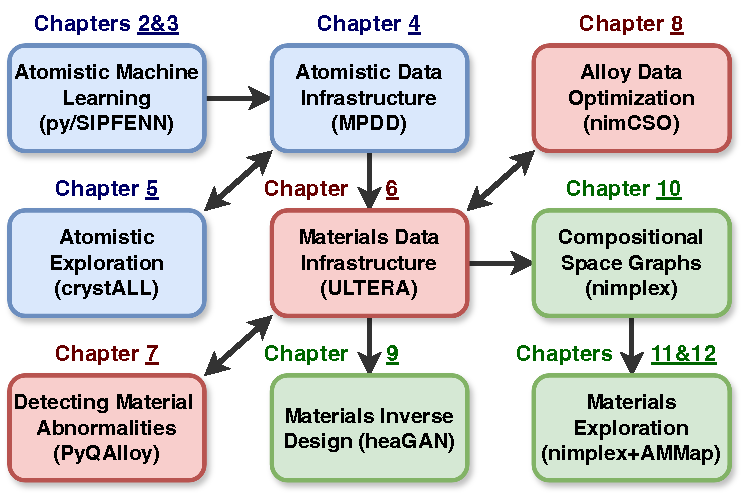
\includegraphics[width=0.7\textwidth]{intro/DissertationOutline.pdf}
    \caption{Schematic outline of this dissertation flowing through 3 overarching types of materials science research. It starts from atomistic treatment (blue) allowing modeling of physical materials (blue) and leading to design (green). For each category, three most significant advancements done in this work have been selected to showcase computational infrastructures and methods to extend our understanding or capabilities.}
    \label{intro:fig:outline}
\end{figure}


\section{Executive Summary} \label{intro:sec:summary}

%%%%%%%%%%
First, Chapter \fullref{chap:sipfenn} introduces fundamental concepts critical to structure-informed modeling of atomic configurations from the perspective of machine learning (ML) modelling and presents design of such models employing artificial neural networks.

In the present paper, we introduce a new neural network-based tool for the prediction of formation energies of atomic structures based on elemental and structural features of Voronoi-tessellated materials. We provide a concise overview of the connection between the machine learning and the true material-property relationship, how to improve the generalization accuracy by reducing overfitting, how new data can be incorporated into the model to tune it to a specific material system, and preliminary results on using models to preform local structure relaxations.

The present work resulted in three final models optimized for (1) highest test accuracy on the Open Quantum Materials Database (OQMD), (2) performance in the discovery of new materials, and (3) performance at a low computational cost. On a test set of 21,800 compounds randomly selected from OQMD, they achieve a mean absolute error (MAE) of 28, 40, and 42 meV/atom, respectively. The second model provides better predictions in a test case of interest not present in the OQMD, while the third reduces the computational cost by a factor of 8.

We collect our results in a new open-source tool called SIPFENN (Structure-Informed Prediction of Formation Energy using Neural Networks). SIPFENN not only improves the accuracy beyond existing models but also ships in a ready-to-use form with pre-trained neural networks and a GUI  interface. By virtue of this, it can be included in DFT calculations routines at nearly no cost.

%%%%%%%%
Next, Chapter \fullref{chap:pysipfenn} expands


Structure-informed materials informatics is a rapidly evolving discipline of materials science relying on the featurization of atomic structures or configurations to construct vector, voxel, graph, graphlet, and other representations useful for machine learning prediction of properties, fingerprinting, and generative design. This work discusses how current featurizers typically perform redundant calculations and how their efficiency could be improved by considering (1) fundamentals of crystallographic (orbits) equivalency to optimize ordered cases and (2) representation-dependent equivalency to optimize cases of dilute, doped, and defect structures with broken symmetry. It also discusses and contrasts ways of (3) approximating random solid solutions occupying arbitrary lattices under such representations.

Efficiency improvements discussed in this work were implemented within \texttt{pySIPFENN} or \textit{python toolset for Structure-Informed Property and Feature Engineering with Neural Networks} developed by authors since 2019 and shown to increase performance from 2 to 10 times for typical inputs. Throughout this work, the authors explicitly discuss how these advances can be applied to different kinds of similar tools in the community.





%%%%%%%
Chapter \fullref{mpdd:sec:mpdd},






%%%%%%%
Chapter \fullref{chap:crystall},






%%%%%%%
Chapter \fullref{chap:ultera}





%%%%%%%
Chapter \fullref{chap:ultera}


Humanity spent the last 5,000 years advancing alloys, first through many empirical breakthroughs and then through a better scientific understanding of the mechanisms at play. The latter requires not only expert knowledge but also the support of experimental datasets. Generally, the limiting factor in such a design approach was the analysis, while data collection was relatively quick. However, in recent years computational data analysis, machine learning (ML), and online literature access are reversing this paradigm, putting more emphasis on the collection of large datasets and building large multi-component CALPHAD databases.
As our community moves towards this large-scale multi-source data collection, additional challenges start to surface, with one of the most critical being the substantial presence of erroneous data. While present in datasets on all alloy classes, this problem is particularly visible in high entropy alloys (HEAs) due to their novelty and complexity. Based on our analysis across several highly regarded HEA datasets and parsing researchers, we estimate a consistent 5-10\% error rate caused by a number of factors, including a lack of standardized notations and general parsing mistakes, such as typos.

\vspace{24pt}
\textit{Figure 1. Schematic of how several methods utilize compositional and property data to detect abnormalities.}\\


To address this challenge, we present a set of open-source Python tools that can be run on alloy datasets to screen them for a variety of abnormalities. They put each data point in a variety of scopes ranging from individual datapoint analysis, through single-study meta-data, to the database as a whole. Depending on method, they can utilize different parts of a datapoint, as shown in Figure 1.
We demonstrate how we deployed these tools in our ULTERA database, developed under the ARPA-E's ULTIMATE program, which collects literature data on (HEAs) to facilitate rapid discovery using forward and inverse design methods [1], with the primary focus on ductility, creep behavior, yield stress, and hardness at elevated temperatures. It is an excellent testing ground due to its size. As of March 2023, ULTERA [2] contains over 6,200 property-datapoints, corresponding to 2,485 unique HEAs collected from 479 literature publications (ultera.org). The database architecture, presented in Figure 2, is an advanced tool itself, allowing automatic real-time integration of the literature data with data from our experiments, generative modeling, predictive modeling, and validations.





%%%%%%%
Chapter \ref{chap:nimplex}

Many disciplines of science and engineering deal with problems related to compositions, ranging from chemical compositions in materials science to portfolio compositions in economics. They exist in non-Euclidean simplex spaces, causing many standard tools to be incorrect or inefficient, which is significant in combinatorically or structurally challenging spaces exemplified by Compositionally Complex Materials (CCMs) and Functionally Graded Materials (FGMs). Here, we explore them conceptually in terms of problem spaces and quantitatively in terms of computational feasibility.

This work implements several essential methods specific to the compositional (simplex) spaces through a high-performance open-source library \texttt{nimplex}. Most significantly, we derive and implement an algorithm for constructing a novel n-dimensional simplex graph data structure, which contains all discretized compositions and all possible neighbor-to-neighbor transitions as pointer arrays. Critically, no distance or neighborhood calculations are performed, instead leveraging pure combinatorics and the ordering in procedurally generated simplex grids, keeping the algorithm $\mathcal{O}(N)$, so that graphs with billions of transitions take seconds to construct on a laptop. Furthermore, we demonstrate how such graph representations can be combined to express path-planning problem spaces and to incorporate prior knowledge while keeping the problem space homogeneous. This allows for efficient deployment of existing high-performance gradient descent, graph traversal search, and other path optimization algorithms.


\section{Software Developed In This Work} \label{intro:sec:software}


\begin{itemize}
    \item 
\end{itemize}



\printbibliography[heading=subbibintoc]